%!TEX root=masterproef.tex

\chapter{Architectuur}
\label{chapter:architectuur}

De oplossingsstrategie bestaat erin om een uitwendige DSL te combineren met
codegeneratie om zo een volledig geautomatiseerde keten te bekomen van
onderzoek tot uitbating. Dit hoofdstuk bekijkt de oplossing vanuit een
architecturaal oogpunt.

Sectie \ref{section:arch-functional} bekijkt de functionaliteit van de
oplossing en identificeert de verschillende functionele componenten met hun
onderlinge relaties. Dit overzicht bepaalt tevens de scope die zal aangehouden
worden in deze masterproef.

Sectie \ref{section:arch-technical} werkt vervolgens deze functionele
architectuur uit in een technische architectuur. Hier wordt het functionele
proces opgedeeld in technische componenten en worden de verschillende interne
informatiestromen, -manipulaties en -opslagvormen ge\"identificeerd.

\section{Functionele architectuur}
\label{section:arch-functional}

Figuur \ref{fig:arch-functional} geeft een overzicht van de voorgestelde
oplossing.

\begin{figure}[ht]
  \centering
  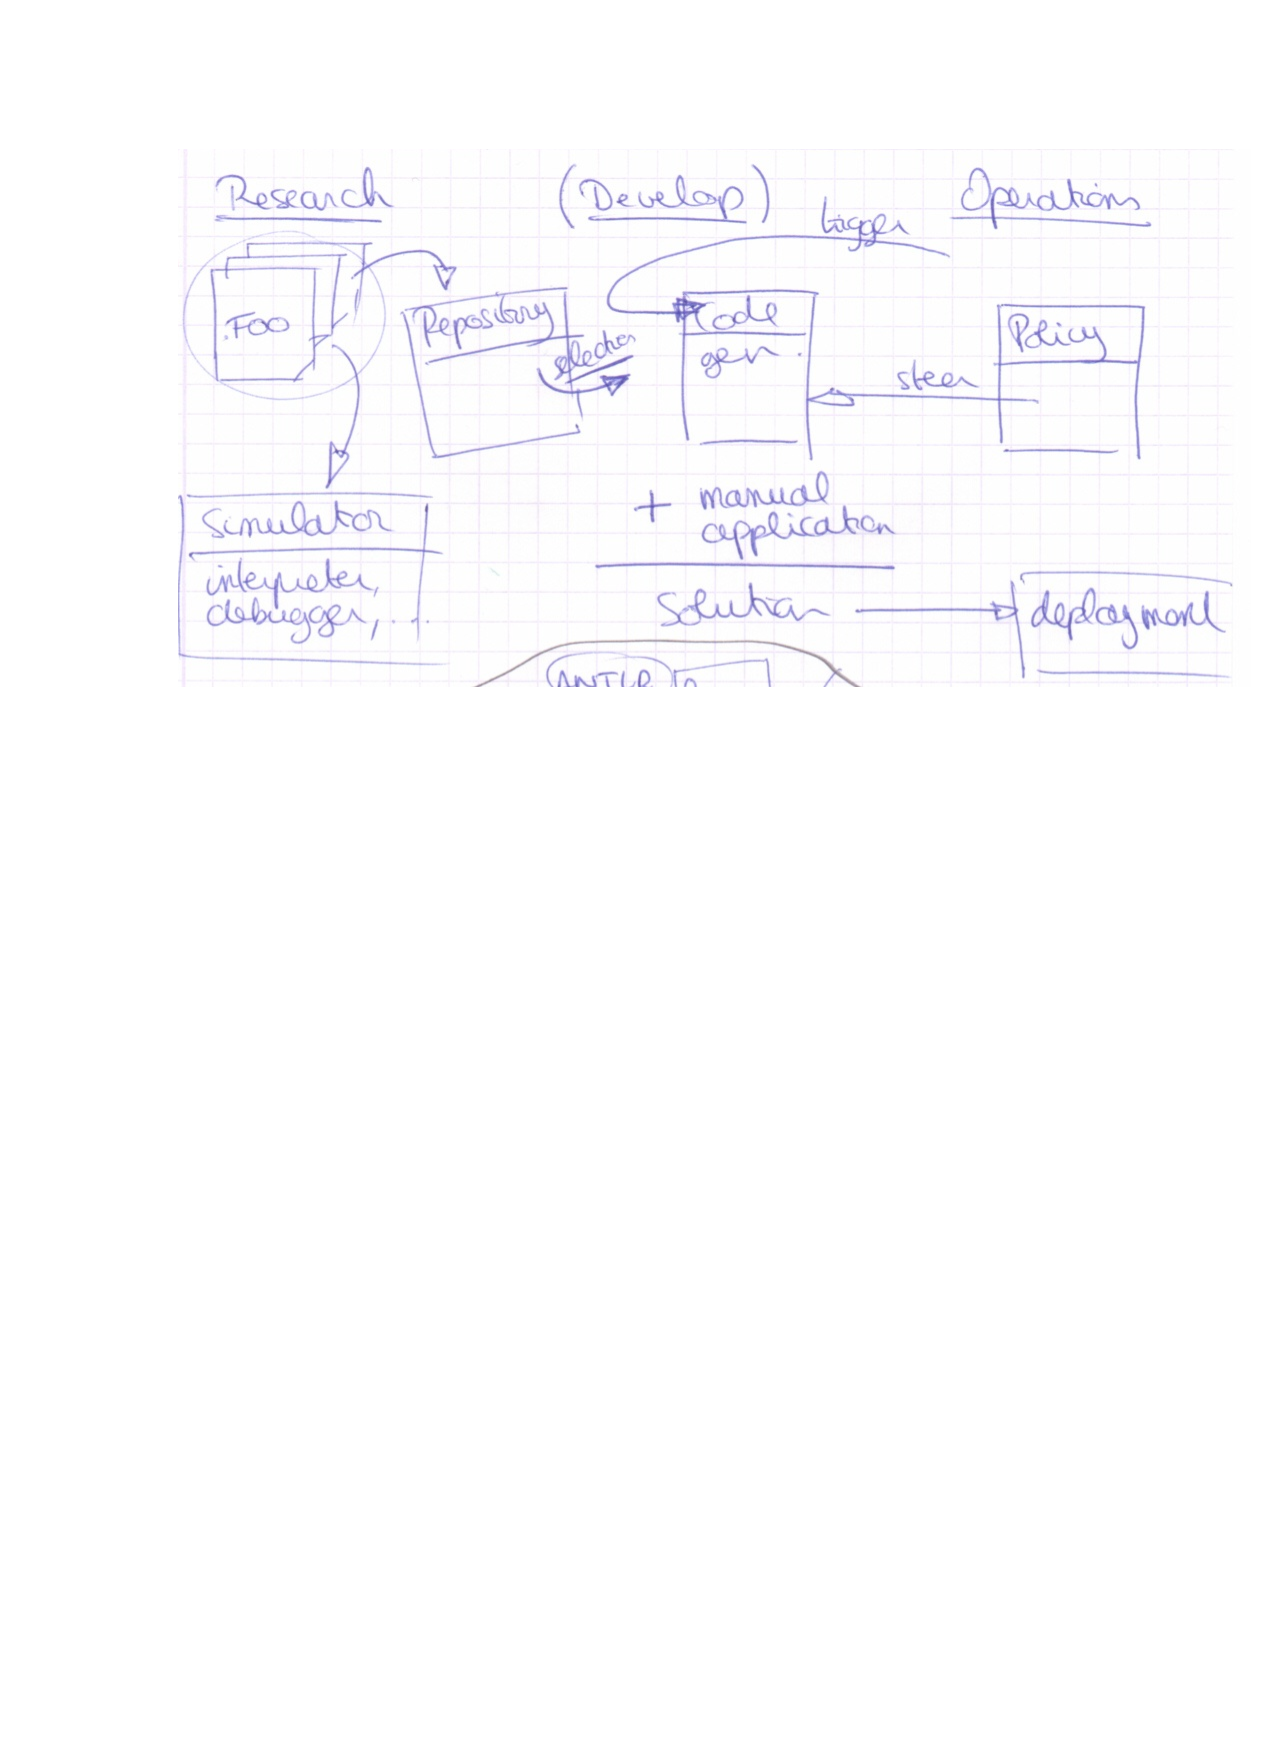
\includegraphics[width=0.9\linewidth]{resources/arch-functional.pdf}
  \caption{Functionele architectuur}
  \label{fig:arch-functional}
\end{figure}

Drie stappen uit het ontwikkelingsproces volgen elkaar op: onderzoek,
ontwikkeling en uitbating.

\begin{description}

    \item[Onderzoek] In deze fase kan een DSL gebruikt worden om het resultaat
    van het onderzoek op formele manier vast te leggen. We stellen hier
    \emph{FOO-lang} voor. Reeds in deze fase kan dit gebruikt worden om verdere
    \emph{analyses}, \emph{simulaties}\dots te doen. Het is tot slot tevens
    mogelijk om een \emph{centrale opslag} te voorzien waar alle
    detectiealgoritmen verzameld kunnen worden en vanwaaruit verder opnieuw
    analyses en simulaties kunnen opgestart worden.
    
    \item[Ontwikkeling] Aan de hand van de formele beschrijvingen kan de
    feitelijke ontwikkeling van het IDS feitelijk vervangen worden door een
    geautomatiseerde \emph{codegeneratie}.
    
    \item[Uitbating] Het wordt zelfs mogelijk om deze codegeneratie te sturen
    vanuit het \emph{beleid} van de uitbating en te integreren in de
    \emph{verspreiding} van het ge\"integreerde systeem.
    
\end{description}

\noindent In de volgende secties belichten we deze aspecten in meer detail.

\subsection{FOO-lang}
\label{subsection:arch-foo-lang}

De eerste belangrijke component van de oplossing is de domeinspecifieke taal,
waarmee detectiealgoritmen beschreven worden. De doelstelling van de taal is om
de functionaliteit zo optimaal mogelijk te organiseren. Hierdoor wordt getracht
om het gebruik van de \mcu en het gebruik van de draadloze radio te beperken.
Deze doelstelling wordt ook weerspiegeld in de naam: Functie Organisatie
Optimalisatie (\emph{Function Organisation Optimisation}), kortweg: FOO-lang.

De belangrijkste doelgroep wat betreft gebruikers, zijn onderzoekers van
inbraakdetectie in het kader van een WSN. Met FOO-lang beschikken zij over een
formele taal om inbraakdetectiealgoritmen te beschrijven.

Het is van primordiaal belang dat de taal zo dicht mogelijk aansluit bij
bestaande kennis en vertrouwde paradigma. Daarom wordt voorgesteld om dicht bij
de programmeertaal C aan te blijven leunen en deze uit te breiden met
constructies die de taal op een hoger niveau van abstractie brengen. Dit hogere
niveau sluit meer aan bij een functionele en platformonafhankelijke
beschrijving.

Om de doelstelling, nl. het genereren van code die betere prestaties laat
optekenen dan eenvoudig manueel samengestelde code, na te streven, is het
belangrijk dat er controle is over de iteratieve aspecten van de algoritmen.
Deze hebben meestal betrekking op de sensorknopen in de nabijheid van de knoop
in kwestie. Door de functionaliteit van het domein te centraliseren rond deze
knopen, is het mogelijk om deze iteraties weg te werken. Door het defini\"eren
van gebeurtenissen waarop kan gereageerd worden met functionaliteit, is het
mogelijk om abstractie te maken van de volledige lijst van sensorknopen en het
algoritme in stukken te breken die als reacties op de gebeurtenissen kunnen
beschreven worden.

Om het functionele karakter verder te onderstrepen is het belangrijk dat zoveel
mogelijk technische aspecten uit de algoritmen geweerd worden. Een typisch
voorbeeld is de typering van variabelen. Typering zal een noodzaak blijken,
maar moet op zijn minst optioneel zijn en indien nodig voorzien worden als een
beperkte set van functionele types. Dit is ook een belangrijke voorwaarde voor
de platformonafhankelijkheid.

\subsection{Centrale opslag}
\label{subsection:arch-repository}

Al deze platformonafhankelijke en formele beschrijvingen van
detectiealgoritmen, kunnen vervolgens samengebracht worden in een centrale
opslagplaats. Het hoeft geen betoog dat hiervoor een website kan voorzien
worden, die als portaal kan dienen. Een heel aantal klassieke voorzieningen
bieden zich hierbij aan: zoekmogelijkheden, gebruiksstatistieken, commentaar,
samenwerkingsmogelijkheden\dots

Allerhande integraties kunnen voorzien worden om op transparante wijze met
zoveel mogelijk de facto standaarddiensten te kunnen samenwerken. Hierbij
denken we aan diensten die opslag van programmacode aanbieden, of meer algemeen
opslag van bestanden, tot processturingsplatformen of probleemopvolgsystemen.

De toegang tot de broncode van de algoritmen moet enerzijds mogelijk zijn via
de eerder visuele website, maar moet zeker geautomatiseerd ge\"integreerd
kunnen worden, zodat bv. compilatieprocessen de laatste versie van een
algoritme kunnen downloaden zonder tussenkomst van een persoon.

\subsection{Codegeneratie}
\label{subsection:arch-codegen}

Het kloppend hart van de oplossing bestaat uit de codegenerator. Deze
accepteert de in FOO-lang geschreven algoritmen en vormt deze om tot
georganiseerde code voor het geselecteerde platform, eventueel voor een gegeven
taal\dots

De generator moet de doelstellingen van de oplossingsstrategie implementeren en
de resulterende code op zo'n manier structureren dat deze minder impact heeft
op de werking van de sensorknoop.

Om een volledig geautomatiseerde werking toe te laten is het belangrijk dat de
aansturing van de generator in zo'n context mogelijk is. De configuratie van de
generator moet via een bestand of aan de hand van oproepparameters
gespecificeerd kunnen worden, zonder verdere menselijke tussenkomst.

\subsection{Uitbating: beleid en verspreiding}
\label{subsection:arch-policy}

Een volledig geautomatiseerde oplossing laat toe om een uitbatingsbeleid te
introduceren op veel fijnere schaal. Het wordt immers mogelijk om zelfs per
sensorknoop een ``persoonlijke'' configuratie te gaan onderhouden, bouwen en
verspreiden.

Hierbij komt de oplossing ook tegemoet aan bv. de nood van sommige algoritmen
om op verschillende soorten knopen verschillende functionaliteit te voorzien.
Vanuit een uitbatingsbeleid is dit een groot voordeel: naast de optimalisatie
van het gebruik van de middelen van \'e\'en knoop, kan nu ook een spreiding
over verschillende knopen helpen om het gemiddeld aantal algoritmen per knoop
te verlagen en zelfs dynamisch op regelmatige tijdstippen te wijzigen.

Gecombineerd met voorzieningen die softwareverspreiding via het draadloze
netwerk (\emph{Over The Air Programming}) (OTAP) toelaten, kan het
gedistribueerde IDS op elk ogenblik gewijzigd worden. Tal van mogelijkheden
ontstaan zo.

\subsection{Ontwikkeling}
\label{subsection:arch-integration}

Naast het IDS is er ook de eigenlijke toepassing die op de sensorknoop zal
ge\"installeerd en uitgebaat worden. Ook deze moet optimaal verwerkt kunnen
worden in het samenstellingsproces.

Een minimale vereiste is dat het generatieproces duidelijke markeringen in de
resulterende code achterlaat, zodat de integratie met de toepassingscode
mogelijk is. Deze markeringen kunnen ook voorzien worden in de vorm van
invoegdirectieven die tijdens het compilatieproces bijkomende bestanden kan
opnemen zonder verdere tussenkomst van een ontwikkelaar.

\subsection{Verdere opportuniteiten}
\label{subsection:arch-opportunities}

Met een centrale opslagplaats en een volledig geautomatiseerde codegeneratie
zijn tal van ondersteunende toepassingen denkbaar.

Een belangrijk voorbeeld voor onderzoekers is een gestandaardiseerde
simulatieomgeving. Deze kan opgebouwd worden met de codegenerator, voorzien van
een implementatie voor een virtueel platform, die bruikbare code genereert voor
de simulatieomgeving. Een integratie zou kunnen bestaan in een implementatie in
Javascript, wat toelaat om de simulatie toe te voegen aan de centrale
opslagplaats en dynamisch verschillende combinaties van algoritmen daaruit te
testen alvorens ze te integreren in een echte omgeving.

\subsection{Scope}
\label{subsection:arch-scope}

De voorgaande hoogniveau functionele analyse toont vooral aan dat met de
basiscomponenten veel andere opportuniteiten in bereik liggen. Het is
belangrijk om deze opportuniteiten in het vizier te houden, zodat er geen
uitgesloten worden door de implementatie.

De minimale set aan basiscomponenten zal in deze masterproef verder uitgewerkt
worden aan de hand van een prototype, enerzijds FOO-lang en anderzijds een
codegenerator met ondersteuning voor \'e\'en combinatie van platform en
programmeertaal. Een centrale opslag en integraties met een beleid of
verspreiding van software worden niet verder uitgewerkt.

\section{Technische architectuur}
\label{section:arch-technical}

Figuur \ref{fig:arch-technical} toont de vertaling van de beoogde functionele
scope naar meer technische componenten. 

\begin{figure}[ht]
  \centering
  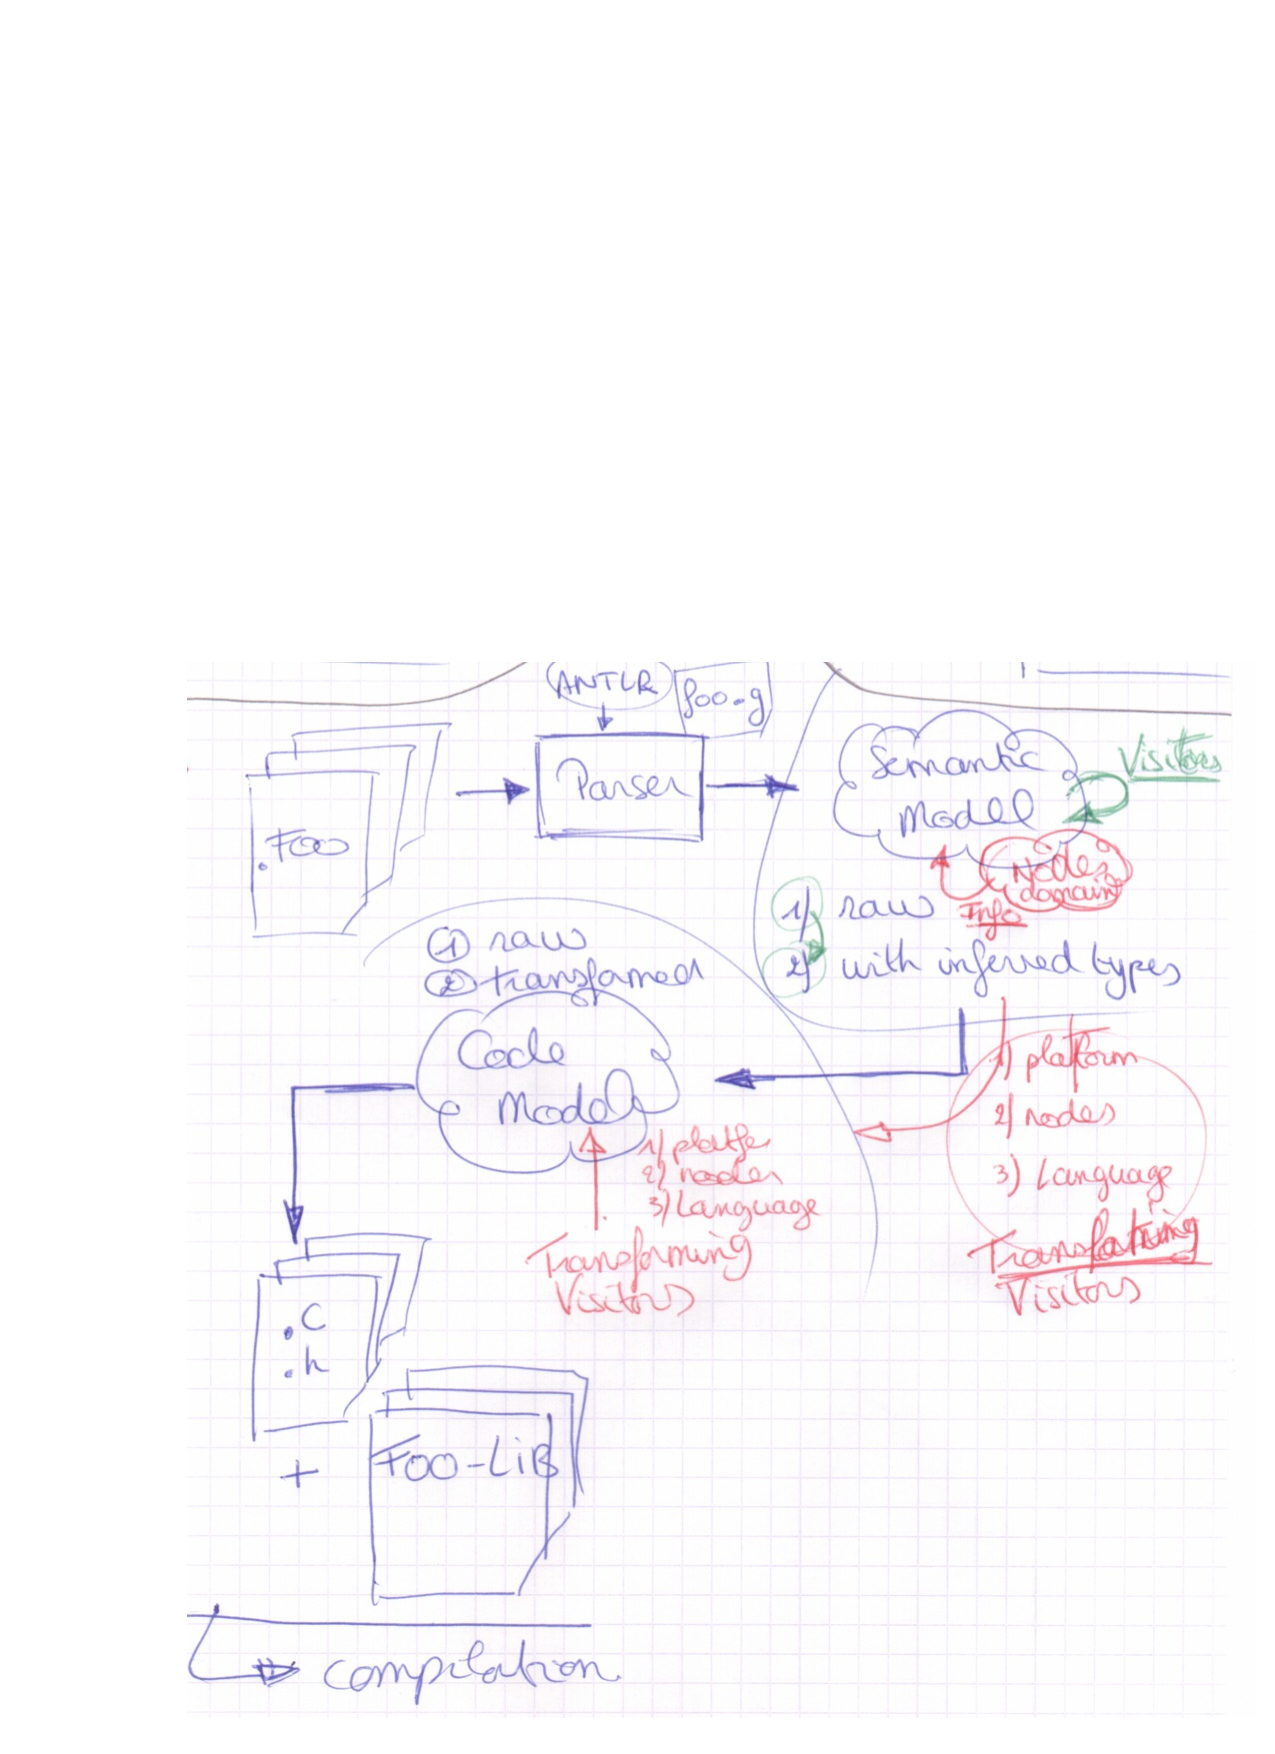
\includegraphics[width=0.9\linewidth]{resources/arch-technical.pdf}
  \caption{Technische architectuur}
  \label{fig:arch-technical}
\end{figure}

\subsection{Parser}

De verwerking verloopt als volgt: een parser analyseert de FOO-lang broncode en
produceert een zgn. abstracte syntax boomvoorstelling (\emph{Abstract Syntax
Tree} (AST). Deze AST wordt vervolgens ingeladen in een \emph{semantisch model}
(SM) \citep{fowler2010domain}.

\subsection{Semantisch model}
\label{subsection:arch-semantic-model}

Een SM bevat de volledige en semantisch correcte voorstelling van de boogde
functionaliteit. In die optiek vertoont het sterke overeenkomsten met een
klassiek domeinmodel \citep{fowler2010domain}, maar aangezien dit laatste
echter veel rijker is aan functionaliteit en een SM typisch meer
informatie-geori\"enteerd is, wordt er een onderscheid gemaakt in de naamgeving.

Het model is volledig ge\"ent op het domein waarvoor het opgebouwd wordt. In
bijlage \ref{appendix:semantic-model} wordt het SM weergegeven. Het bevat alle
functionele aspecten die nodig geacht worden om algoritmen in het domein
functioneel te beschrijven.

Op het hoogste niveau herkennen we het model als alles omvattende entiteit.
Hieronder worden de modules geplaatst, die overeenkomen met telkens \'e\'en
algoritme. Modules bevatten functionaliteit in de vorm van
functiebeschrijvingen.

Het centrale concept is dat van de uitvoeringsstrategie (\emph{Execution
Strategy})\footnote{Er is geopteerd om in de programmacode van de generator een
Engelstalige terminologie aan te houden.}. Deze verbindt functionaliteit met de
knopen. Twee soorten strategie\"en zijn voorzien: een reactie op een
gebeurtenis (\emph{Handler}) en een weerkerende actie (\emph{Every}).

Op een lager niveau wordt de functionaliteit beschreven aan de hand van een
syntax die nauw aansluit bij deze van de programmeertaal C. Deze is uitgebreid
met constructies van een hoger abstractieniveau om op een functionelere manier
om te kunnen gaan met de entiteiten uit het domein.

\subsection{Type deductie en andere transformaties}

Door middel van verschillende transformaties wordt dit SM vervolledigd. Een
eerste stap is het deduceren van ontbrekende types. Het resultaat is een
volledig getypeerd SM en garandeert een correcte behandeling, eventueel in het
kader van een sterk getypeerde programmeertaal, zoals C.

Een tweede stap is een vertaling van het SM naar een \emph{code model} (CM).
Dit CM staat dichter bij de uiteindelijk te genereren code en is meer technisch
van aard. Deze vertaling is het resultaat van verschillende transformaties
uitgevoerd op het SM door o.a. de specifieke implementatie voor het platform en
het domein.

\subsection{Code model}
\label{subsection:arch-code-model}

Via de verschillende transformaties wordt het SM omgezet in een CM. Deze
overstap vertaalt in essentie de functionele concepten naar overeenkomstige
patronen in een semantiek die direct aanleunt bij programmeertalen.

Het code model voorziet een hi\"erarchie van een compilatie unit, met daaronder
modules en binnen elke module secties. Deze hi\"erarchie is een abstracte
voorstelling van respectievelijk de gehele compilatie, de functionele modules
en de bestanden waaruit die modules opgebouwd zullen worden. In termen van de
programmeertaal C is dit het geheel van C en aanverwante bestanden, het concept
van een C module en op het laagste niveau de effectieve C en hoofding bestanden.

Een sectie bestaat dan uit \'e\'en of meerdere codeconstructies:
functiedeclaraties, expressies, statements\dots Deze codeconstructies zijn
rijker dan bv. de programmeertaal C. Het zal de taak zijn van opeenvolgende
transformaties om deze niet-ondersteunde constructies voor een bepaald platform
en/of programmeertaal om te vormen naar constructies die wel door de taal of
het platform worden aangeboden.

\subsection{Codegeneratie}

De laatste stap in het proces bestaat uit de eigenlijke generatie van
programmacode. Deze vertrekt van het CM en is ook samengesteld met
transformaties. Hier is de beoogde programmeertaal de belangrijkste bron voor
transformaties. Het resultaat is een CM dat \'e\'en-op-\'e\'en vertaalbaar is
naar programmacode en zo eigenlijk kan beschouwd worden als een AST.
